\newpage

\section{Detekcja twarzy} \label{section:face_detection}
\_\_\_\_\_\_ TODO \_\_\_\_\_\_ 
\subsection{Cascading Classifier}
\_\_\_\_\_\_ TODO \_\_\_\_\_\_ 
\subsubsection{Haar Cascade}
\_\_\_\_\_\_ TODO \_\_\_\_\_\_ 
\subsubsection{LBP Cascade}
\_\_\_\_\_\_ TODO \_\_\_\_\_\_ 



\subsection{Deep Neural Network}
Głębokie sieci neuronowe bazujące na różnych modelach dostają na wejście obraz. Na ich podstawie tworzą plamki o ustalonej wielkości, a następnie przepuszczają je przez kolejne warstwy celem wykrycia pożądanych obiektów. 
\par
W projekcie zostanie wykorzystany do tego pakiet pakiet \textit{OpenCV-contrib} \cite{opencv_contirb} zawierający implementację DNN.
\par
Jednym z modeli dostępnych do detekcji twarzy przy pomocy głębokich sieci neuronowych są modele Caffe (\textit{Convolutional Architecture for Fast Feature Embedding}) \cite{jia2014caffe}. Aktualnie używany w projekcie wzorzec caffe to \textit{res10{\_}300x300{\_}ssd{\_}iter{\_}140000{\_}fp16} \cite{caffemodel_res10}.


\subsection{Filtrowanie wyników}
\label{section:face_detection_filter}

Użyte algorytmy mogą dawać w wyniku błędnie określone obszary twarzy. Z tego względu zwróconą tablicę obszarów poddaje filtrowaniu.
\par
Etapy filtracji obrazów:

\begin{itemize}
    \item Na początku odrzucam obszary, których środek znajduje się poza ustalonym pionowym obszarem (przyjąłem przedział [0.25, 0.75] szerokości). Wynika to z założeń, że osoba używająca telefonu, korzysta z niego patrząc na wprost, a nie z boku. Natomiast odchył od pionu to indywidualne preferencje - dlatego nie określam poziomego obszaru. (patrz \hyperref[{fig:face_boundary}]{\textit{Rysunek \ref{fig:face_boundary}}})

    \begin{figure}[!h]
        \begin{center}
            \subfigure[Przed filtrowaniem zależnym od położenia]{\label{fig:face_boundary_before}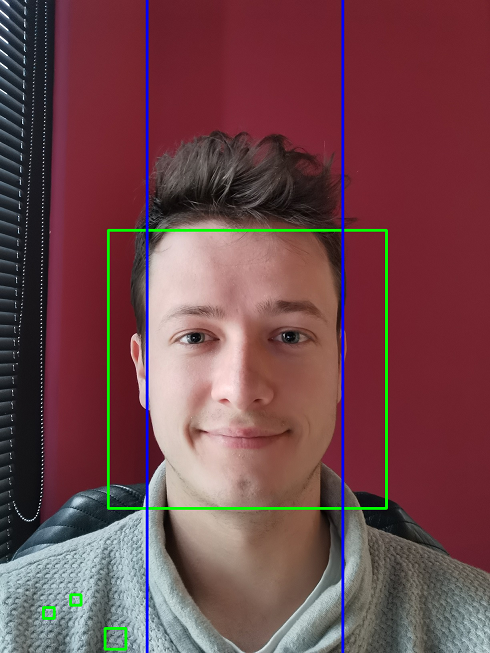
\includegraphics[scale=0.3]{img/face_section/face_filter_boundary_1.png}}
            \hspace{8mm}
            \subfigure[Po filtrowaniu]{\label{fig:face_boundary_after}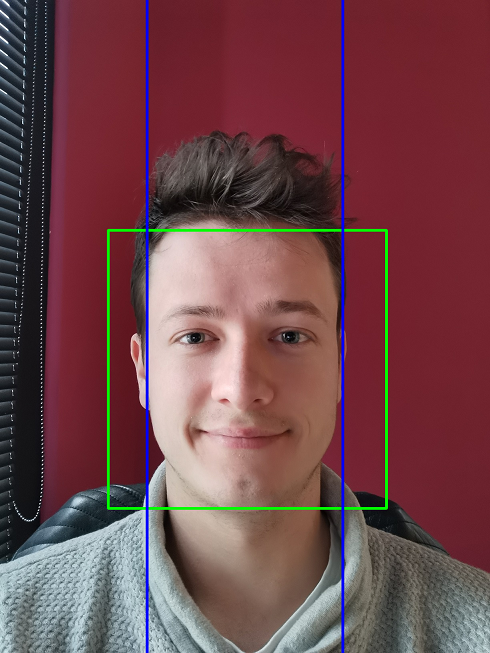
\includegraphics[scale=0.3]{img/face_section/face_filter_boundary_2.png}}
        \end{center}
        \caption{Działanie filtrowania detekcji twarzy w oparciu o położenie twarzy w centralnej części zdjęcia.}
        \label{fig:face_boundary}
    \end{figure}
    
    \item Kolejnym etapem jest odrzucenie tych detekcji, które wychodzą zbyt daleko poza zdjęcie Jeśli którykolwiek z boków prostokąta wystaje pionowo/poziomo o odległość większą niż $10\%$ odpowiednio wysokości/szerokości to zostaje odrzucony. (patrz \hyperref[{fig:face_out}]{\textit{Rysunek \ref{fig:face_out}}})
    
    \begin{figure}[!h]
        \begin{center}
            \subfigure[Przed filtrowaniem zależnym od wystawania poza obraz]{\label{fig:face_out_before}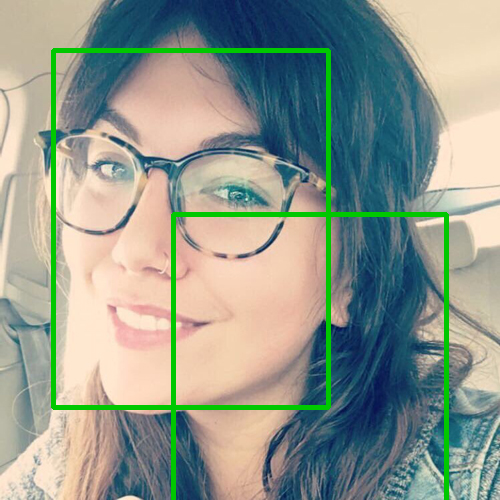
\includegraphics[scale=0.25]{img/face_section/face_filter_out_before.png}}
            \hspace{8mm}
            \subfigure[Po filtrowaniu]{\label{fig:face_out_after}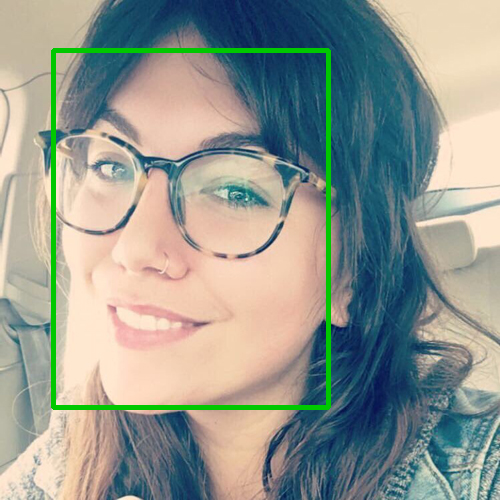
\includegraphics[scale=0.25]{img/face_section/face_filter_out_after.png}}
        \end{center}
        \caption{Działanie filtrowania detekcji twarzy w oparciu o odległość wykrytego obszaru poza zdjęcie.}
        \label{fig:face_out}
    \end{figure}
    
    \item Z pozostałych obszarów wybieram ten, który zajmuje największą powierzchnię. Taki wybór motywuję własnymi obserwacjami zachowania algorytmów detekcji twarzy oraz tym, że głowa użytkownika telefonu na obrazie z kamery przedniej zajmuję większą część płaszczyzny, ponieważ korzystając z urządzenia nie trzymamy go bardzo daleko od siebie. (patrz \hyperref[{fig:face_size}]{\textit{Rysunek \ref{fig:face_size}}})
    
    \begin{figure}[!h]
        \begin{center}
            \subfigure[Przed filtrowaniem zależnym od wielkości]{\label{fig:face_size_before}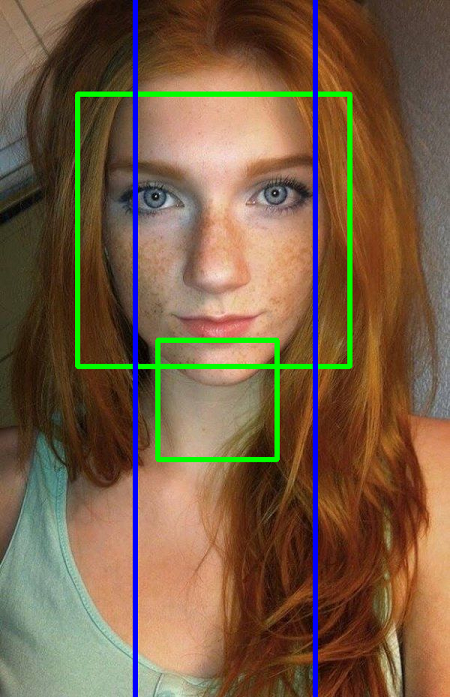
\includegraphics[scale=0.3]{img/face_section/face_filter_size_1.png}}
            \hspace{8mm}
            \subfigure[Po filtrowaniu]{\label{fig:face_size_after}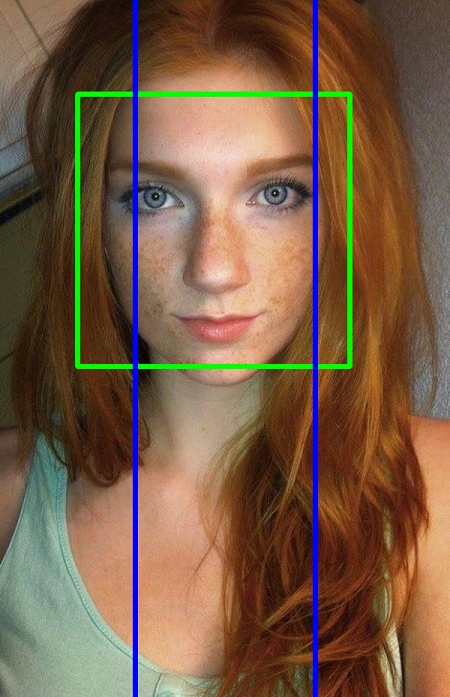
\includegraphics[scale=0.3]{img/face_section/face_filter_size_2.png}}
        \end{center}
        \caption{Działanie filtrowania detekcji twarzy w oparciu o wielkość wykrytego obszaru. Źródło zdj.: \cite{readheadPortrait1}}
        \label{fig:face_size}
    \end{figure}
    
    
    
\end{itemize}


\section{Porównanie algorytmów detekcji twarzy}

\_\_\_\_\_\_ TODO \_\_\_\_\_\_ 

\subsection{Testowanie na statycznych zdjęciach}

Pierwszy etap testowania algorytmów detekcji twarzy będzie bazował na statycznych zdjęciach z głównego datasetu (patrz rozdz. \hyperref[section:dataset]{\textit{\ref{section:dataset}.Dataset}}). Pozwoli to przetestować na jednakowych danych wszystkie metody pod względem ich skuteczności wykrywania docelowych obszarów w różnych warunkach oraz uzyskać miarodajne wyniki.

\subsubsection{Oczekiwany wynik}

Każde zdjęcie z datasetu do tego etapu zostało opisane przez dwa prostokąty między którymi powinna się znaleźć wykryta przez algorytm twarz. Obszar ten został dobrany w następujący sposób:

\begin{itemize}
    \item Wewnętrzna część obejmuje minimalny obszar, na którym znajdują się brwi, oczy, nos i usta.
    \item W zewnętrznym prostokącie powinna znaleźć się cała twarz. Powiększony jest on o pewną tolerancję. 
\end{itemize}

\begin{figure}[!h]
    \begin{center}
        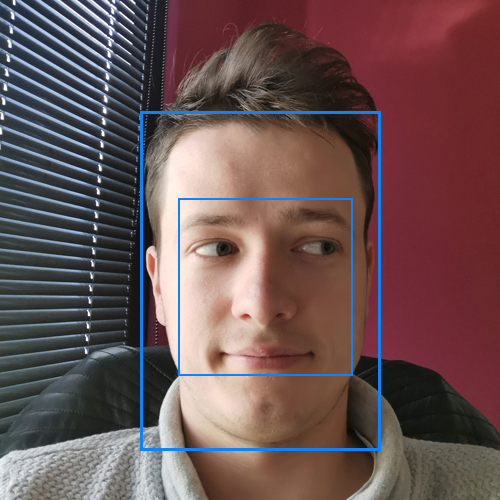
\includegraphics[scale=0.3]{img/face_section/face_test_expected.jpg}
        \caption{Oczekiwany obszar detekcji twarzy. }
        \label{fig:face_test_expected}
    \end{center}
\end{figure}

\subsubsection{Sposób testowania}

Dla każdego algorytmu zostanie przeprowadzone testy na zestawach obrazów o następujących rozdzielczościach i przestrzeniach barw:

\begin{itemize}
    \item 300x300 RGB
    \item 500x500 RGB
    \item 300x300 skala szarości
    \item 500x500 skala szarości
\end{itemize}

W przypadku \textit{DNN Caffe} nie jest możliwe przeprowadzenie badań dla zdjęć w skali szarości, ponieważ wymaga on obrazu z trzema kanałami barw.

\subsubsection{Zbierane dane}

Dla każdego rodzaju testu i algorytmu zostaną zebrane następujące dane:

\begin{itemize}
    \item \textbf{Prawidłowe detekcje} - suma perfekcyjnych i częściowo dobrych detekcji
    \item \textbf{Perfekcyjne detekcje} - jeśli wykryty obszar w pełni znajduje się pomiędzy oczekiwanym prostokątami
    \item \textbf{Częściowo dobre detekcje} - jeśli są krawędzie, które znajdują się poza oczekiwanym obszarem, ale w zadowalającej odległości (patrz niżej - \hyperref[{uwaga:czesciowo_dobry}]{\textit{Uwaga 1.}})
    \item \textbf{Z 3 na 4 krawędzie perfekcyjne detekcje} - jeśli tylko jedna krawędź znajduje się poza oczekiwanym obszarem w zadowalającej odległości (patrz niżej - \hyperref[{uwaga:3_4_perfekcyjny}]{\textit{Uwaga 2.}})
    \item \textbf{Złe detekcje} - jeśli twarz nie została wykryta lub wskazany obszar jest niezadowalający
    \item \textbf{Twarze niewykryte} - jeśli całkowicie nie udało się wykryć twarzy (patrz niżej - \hyperref[{uwaga:dodatkowy_zle}]{\textit{Uwaga 3.}})
    \item \textbf{Średnia procentowa odległość błędnych krawędzi} - wyrażony w procentach średni stosunek odległości krawędzi do szerokości/wysokości maksymalnego dopuszczalnego obszaru dla błędnie wykrytych stron
    \item \textbf{Średni czas przetwarzania jednego zdjęcia} - wyrażony w sekundach czas potrzebny na przetworzenie jednego zdjęcia przez daną  metodę (patrz niżej - \hyperref[{uwaga:ilosc_powtorzen}]{\textit{Uwaga 4.}})
\end{itemize}

\textit{Uwaga 1.}\label{uwaga:czesciowo_dobry} Obszar uznany jest za częściowo dobry jeśli żadna krawędź nie jest oddalona o więcej niż $1.2x$ i maksymalnie jedna oddalona jest o długość z przedziału $[1.1x, 1.2x]$. Odległość $x$ to szerokość lub wysokość (zależnie od krawędzie) maksymalnego oczekiwanego obszaru twarzy.
\par
\textit{Uwaga 2.}\label{uwaga:3_4_perfekcyjny} Obszar zaliczony jest do grupy 3/4 perfekcyjnych detekcji, jeśli 3 krawędzie znajdują się w oczekiwanym obszarze, a czwarta odchylona od normy w przedziale $[1.0x, 1.2x]$.
\par 
\textit{Uwaga 3.}\label{uwaga:dodatkowy_zle} Dodatkowy podział złej detekcji na niewykryte twarze wynika z faktu, że metody oparte o \textit{Cascasding Classifier} na wyjściu podają obszar kwadratowy i przy rozciągniętej lub pochylonej twarzy boczne obszary mogą być bardzo oddalone od oczekiwanej wartości, ale dalej wykryć twarz. 
\par
\textit{Uwaga 4.}\label{uwaga:ilosc_powtorzen} Celem miarodajnego wyniku czasu przetwarzania każdy test zostanie przeprowadzony 20 razy, a wyniki uśrednione.

\subsubsection{Wyniki}
\label{section:face_main_test}

\begin{table}[!h]
\label{tab:face_detect_result_RGB}
\centering
\caption{Wynik porównania algorytmów detekcji twarzy dla obrazów RGB}
\resizebox{\textwidth}{!}{%
\begin{tabular}{|c|c|c|c|c|c|c|c|c|}
\hline
 &
  \textbf{\begin{tabular}[c]{@{}c@{}}Prawidłowa\\ detekcja\end{tabular}} &
  \textbf{\begin{tabular}[c]{@{}c@{}}Perfekcyjna\\ detekcja\end{tabular}} &
  \textbf{\begin{tabular}[c]{@{}c@{}}Częściowa\\ dobra\\ detekcja\end{tabular}} &
  \textbf{\begin{tabular}[c]{@{}c@{}}3/4\\ krawędzie\\ perfekcyjne\end{tabular}} &
  \textbf{\begin{tabular}[c]{@{}c@{}}Zła\\ detekcja\end{tabular}} &
  \textbf{\begin{tabular}[c]{@{}c@{}}Niewykryte\\ twarze\end{tabular}} &
  \textbf{\begin{tabular}[c]{@{}c@{}}Średnia\\ odległość\\ złych\end{tabular}} &
  \textbf{\begin{tabular}[c]{@{}c@{}}Średni czas \\ przetwarzania\\ pojedynczego\\ zdjęcia\end{tabular}} \\ \hline\hline
\textbf{Haar Cascade 500x500} &
  69 &
  4 &
  65 &
  32 &
  11 &
  9 &
  6,07 \% &
  0,072 s \\ \hline
  
\textbf{Haar Cascade 300x300} &
 68 &
  5 &
  63 &
  33 &
  12 &
   9 &
  6,29 \% &
  0,028 s \\ \hline
  
  \textbf{LBP Cascade 500x500} &
  58 &
  4 &
  54 &
  29 &
  22 &
  22 &
  6,22\% &
  0,039 s \\ \hline
  
  \textbf{LBP Cascade 300x300} &
  61 &
  4 &
  57 &
  34 &
  19 &
  17 &
  6,29 \% &
  0,014 s \\ \hline
  
\textbf{DNN Caffe 500x500} &
  80 &
  68 &
  12 &
  11 &
  0 &
  0 &
  5,49 \% &
  0,079 s \\ \hline
  
\textbf{DNN Caffe 300x300} &
  80 &
  62 &
  18 &
  18 &
  0 &
  0 &
  4,87 \% &
  0,073 s \\  \hline
  
  \hline
\end{tabular}%
}
\end{table}

\begin{table}[!h]
\label{tab:face_detect_result_GRAY}
\centering
\caption{Wynik porównania algorytmów detekcji twarzy dla obrazów w skali szarości}
\resizebox{\textwidth}{!}{%
\begin{tabular}{|c|c|c|c|c|c|c|c|c|}
\hline
 &
  \textbf{\begin{tabular}[c]{@{}c@{}}Prawidłowa\\ detekcja\end{tabular}} &
  \textbf{\begin{tabular}[c]{@{}c@{}}Perfekcyjna\\ detekcja\end{tabular}} &
  \textbf{\begin{tabular}[c]{@{}c@{}}Częściowa\\ dobra\\ detekcja\end{tabular}} &
  \textbf{\begin{tabular}[c]{@{}c@{}}3/4\\ krawędzie\\ perfekcyjne\end{tabular}} &
  \textbf{\begin{tabular}[c]{@{}c@{}}Zła\\ detekcja\end{tabular}} &
  \textbf{\begin{tabular}[c]{@{}c@{}}Niewykryte\\ twarze\end{tabular}} &
  \textbf{\begin{tabular}[c]{@{}c@{}}Średnia\\ odległość\\ złych\end{tabular}} &
  \textbf{\begin{tabular}[c]{@{}c@{}}Średni czas \\ przetwarzania\\ pojedynczego\\ zdjęcia\end{tabular}} \\ \hline \hline
\textbf{Haar Cascade 500x500} &
  69 &
  4 &
  65 &
  31 &
  11 &
  9 &
  6,40 \% &
  0,073 s \\ \hline

\textbf{Haar Cascade 300x300} &
  67 &
  4 &
  63 &
  34 &
  13 &
  9 &
  6,43 \% &
  0,028 s \\ \hline
  
\textbf{LBP Cascade 500x500} &
  60 &
  5 &
  55 &
  30 &
  20 &
  17 &
  6,17 \% &
  0,038 s \\ \hline
  
\textbf{LBP Cascade 300x300} &
  60 &
  4 &
  56 &
  31 &
  20 &
  17 &
  6,65 \% &
  0,013 s \\ \hline
  
\textbf{DNN Caffe 500x500} &
  nd. &
  nd. &
  nd. &
  nd. &
  nd. &
  nd. &
  nd. &
  nd. \\ \hline
  
\textbf{DNN Caffe 300x300} &
  nd. &
  nd. &
  nd. &
  nd. &
  nd. &
  nd. &
  nd. &
  nd. \\ \hline
  
  \hline
\end{tabular}%
}
\end{table}


Metoda \textit{Haar Cascade} daje średnio $\sim69/80$ $(86\%)$ dobrych detekcji. Jest to dosyć przeciętny wynik. Na taki rezultat składa się kilka problemów tej metody. Nie radzi sobie ona dobrze z częściowo zakrytymi twarzami lub gdy głowa jest pochylona w bok. Kolejnymi czynnikiem wpływającym negatywnie na detekcje jest światło - problem z wykrywaniem występuje gdy zdjęcie jest zbyt jasne, twarz oświetlona lub źródło światła świeci prosto w obiektyw. Na plus tej metody można zapisać małą ilość zwróconych przez nią dodatkowych, błędnych obszarów, które musiały zostać odfiltorwane.

\par
\textit{Cascading Classifier} bazując na modelu \textit{LBP} miał najgorsze wyniki detekcji twarzy, na poziomie $\sim60/80$ $(75 \%)$. Jednak co zwraca uwagę to fakt, że bardzo duży odsetek twarzy nie został w ogóle wykryty. Występują tu te same problemy co w \textit{Haar Cascade}, ale dodatkowo algorytm nie radzi sobie gdy twarz zajmuje prawie całe zdjęcie.

\par
Najlepszy wynik detekcji uzyskał bezdyskusyjnie \textit{DNN Caffe}. Fakt, że w każdym z dwóch testów wykrył on $100 \%$ twarzy robi wrażenie. Co więcej perfekcyjne detekcje były na poziomie $\sim65/80$ $(81,25 \%)$. Nie występują tu problemy takie jak w poprzednich algorytmach. Radzi sobie on dobrze w złych warunkach oświetleniowych. Częściowe zakrycie twarzy nie wpływa na detekcję. Wykrywa on dobrze zarówno pochylone jak i odwrócone twarze. Jedyną negatywnym zjawiskiem, które zaobserwowałem w tej metodzie to zwracanie wielu dodatkowych obszarów, które są błędne. Zastosowanie filtrowania pozwoliło jednak odrzucić wszystkie błędne obszary.

\vspace{5mm}
Różnica w procencie perfekcyjnych detekcji pomiędzy \textit{DNN Caffe}, a \textit{LBP} i \textit{Haar} wynika z rodzaju obszarów zwracanych przez te algorytmy. Metoda oparta na głębokich sieciach neuronowych zwraca prostokąt o dowolnym stosunku boków, natomiast druga grupa zwraca kwadrat. Dzięki temu \textit{DNN} lepiej dopasowuję się do kształtu twarzy niż \textit{Cascading Classifier}.

\vspace{5mm}

Najszbyszy okazał się algorytm operujący na modelu \textit{LBP}. \textit{DNN Caffe} dla zdjęć $500x500$  był porównywalnie szybki jak \textit{Haar Cascade}, natomiast już w przypadku $300x300$ około $2.5$ razy wolniejszy.
\par
Co ciekawe i warte odnotowania to fakt, że algorytm \textit{DNN} przetwarzał prawie tak samo szybko obie rozdzielczości zdjęć. Można wysnuć tezę, że dla tej metody wielkość obrazu nie ma wpływu na szybkość przetwarzania. Ze względu, że taka właściwość może okazać się przydatna w perspektywie dalszych etapów projektu, zamierzam zbadać tę zależność w następnym rozdziale.

\vspace{5mm}

Zmiana detekcji z trójkanałowej RGB na skale szarości nie przyniosło żadnej zmiany zarówno w skuteczności algorytmów, jak również nie skróciło czasu detekcji.

\subsection{Dodatkowe testy \textit{DNN Caffe}}

\subsubsection{Wpływ wielkości zdjęcia na czas przetwarzania}

\begin{table}[!h]
\label{tab:face_dnn_speed}
\centering
\caption{Wpływ rozdzielczości zdjęcia na detekcję DNN}
\resizebox{\textwidth}{!}{%
\begin{tabular}{|c|c|c|c|c|c|}
\hline
 &
  \textbf{\begin{tabular}[c]{@{}c@{}}Prawidłowe\\ detekcje\end{tabular}} &
  \textbf{\begin{tabular}[c]{@{}c@{}}Perfekcyjne\\ detekcje\end{tabular}} &
  \textbf{\begin{tabular}[c]{@{}c@{}}Częściowo\\ dobre\\ detekcje\end{tabular}} &
  \textbf{\begin{tabular}[c]{@{}c@{}}Średni czas\\ przetwarzania \\ pojedynczej iteracji\end{tabular}} &
  \textbf{\begin{tabular}[c]{@{}c@{}}Średni czas \\ przetwarzania\\ pojedynczego\\ zdjęcia\end{tabular}} \\ \hline
\textbf{300x300} &
  80 &
  62 &
  18 &
  5,148 s &
  0,064 s \\ \hline
  
\textbf{500x500} &
  80 &
  68 &
  12 &
  5,239 s &
  0,065 s \\ \hline
  
\textbf{1000x1000} &
  80 &
  67 &
  13 &
  5,29 s &
  0,066 s \\ \hline
  
  \textbf{2000x2000} &
  80 &
  65 &
  15 &
  4,988 s &
  0,062 s \\ \hline
 
  \hline
\end{tabular}%
}
\end{table}

Test ten potwierdza postawioną przeze mnie wcześniej tezę, że wielkość zdjęcia nie ma wpływu na szybkość przetwarzania algorytmu \textit{DNN Caffe}. Testy w każdej rozdzielczości zostały wykonane mniej więcej w tym samym czasie, a różnica zapewne jest skutkiem obciążenia urządzenia w danej chwili i jest pomijalna.\\
Prawdopodobnie wynika to z faktu, że metoda ta tworzy na podstawie zdjęcia wejściowego plamki o podanej wielkości niezależnie od rozdzielczości. W zaimplementowanym algorytmie jest to rozmiar 300x300. Dzięki temu zawsze ma on do przetworzenia taką samą ilość danych, więc czas powinien być w przybliżeniu stały.

\textit{Uwaga}. Różncia czasów DNN między tym testem, a poprzednim (\hyperref[{section:face_main_test}]{\textit{patrz rozdz. \ref{section:face_main_test}.Wyniki}}) prawdopodobnie wynika z jróżnych obciążeń telefonu w danym momencie.

\subsubsection{Porównanie precyzji detekcji zależnie od sposóbu filtrowania}

Metoda oparta na głębokich sieciach neuronowych na wyjściu zwraca wiele obszarów wraz ze wskaźnikiem pewności detekcji. Im większy współczynnik tym w teorii większa szansa, że jest to obiekt, który chcieliśmy wykryć.
\par
Z tego powodu postanowiłem porównać autorskie filtrowanie opisane wcześniej (patrz rozdz. \hyperref[{section:face_detection_filter}]{\textit{\ref{section:face_detection_filter}.Filtrowanie wyników}}) i wybór detekcji z największym procentem pewności.
\par

\begin{table}[!h]
\label{tab:face_filter_test}
\centering
\caption{Wynik porównania sposobów filtrowania detekcji twarzy algorytmem DNN Caffe na zbiorze danych.}
\resizebox{\textwidth}{!}{%
\begin{tabular}{|c|c|c|c|c|c|c|}
\hline
 &
  \textbf{\begin{tabular}[c]{@{}c@{}}Prawidłowe\\ detekcje\end{tabular}} &
  \textbf{\begin{tabular}[c]{@{}c@{}}Perfekcyjne\\ detekcje\end{tabular}} &
  \textbf{\begin{tabular}[c]{@{}c@{}}Częściowo\\ dobre\\ detekcje\end{tabular}} &
  \textbf{\begin{tabular}[c]{@{}c@{}}3/4\\ krawędzie\\ perfekcyjnie\end{tabular}} &
  \textbf{\begin{tabular}[c]{@{}c@{}}Złe\\ detekcje\end{tabular}} &
  \textbf{\begin{tabular}[c]{@{}c@{}}Niewykryte\\ twarze\end{tabular}}  \\ \hline \hline
\textbf{Autorskie filtrowanie 300x300} &
  80 &
  62 &
  18 &
  18 &
  0 &
  0  \\ \hline
  
\textbf{Autorskie filtrowanie  500x500} &
  80 &
  68 &
  12 &
  11 &
  0 &
  0  \\ \hline
  
\textbf{Najwyższy współczynnik pewności 300x300} &
  76 &
  58 &
  18 &
  18 &
  4 &
  4  \\ \hline

  \textbf{Najwyższy współczynnik pewności 500x500} &
  76 &
  64 &
  12 &
  11 &
  4 &
  4  \\ \hline
 
  \hline
\end{tabular}%
}
\end{table}


Jak widać zaproponowana przeze mnie wcześniej sekwencja filtrowania wykrytych obszarów daje lepsze rezultaty niż wybór najwyższego współczynnika pewności.


\subsection{Testowanie na obrazie z kamery na żywo}

\_\_\_\_\_\_ TODO \_\_\_\_\_\_ 